\documentclass[handout]{beamer}
\usepackage{multicol}
\everymath{\displaystyle}
\mode<presentation>
{\usetheme{Warsaw}\setbeamercovered{dynamic}}
\usecolortheme{crane}
\usepackage{beamerfoils}
\pgfdeclareimage[height=1in]{university-logo}{ISULogo}
\logo{\pgfuseimage{university-logo}}
\setbeamertemplate{navigation symbols}{}
\title[\S2]{Section 2\\Theoretical probability}
\author{Dr Marcus Bishop}
\subject{Math 104}
\beamerdefaultoverlayspecification{<+->}
\theoremstyle{definition}
\newtheorem{remark}{Remark}
\newtheorem{impact}{Impact}
\newtheorem{notation}{Notation}
\usepackage{arev}
\begin{document}
\begin{frame}\titlepage\end{frame}
\LogoOff

\begin{frame}{Equally likely outcomes}
\begin{definition} If each outcome of experiment
as likely to occur as any other, outcomes called
\alert{equally likely}
\end{definition}
\begin{example}
Outcomes $1,2,3,4,5,6$ of rolling die equally likely
\end{example}
\begin{example}
Outcomes H,T of flipping coin equally likely
\end{example}
\begin{example}
\begin{itemize}
\item Experiment: roll two dice and add results
\item Outcomes 2,3,\ldots,12 \alert{not} equally likely!
\end{itemize}
\end{example}
\end{frame}

\begin{frame}{Example}
\begin{itemize}
\item All possible outcomes of rolling two dice:
\[\begin{array}{llllll}
\left(1,1\right)&
\left(1,2\right)&
\left(1,3\right)&
\left(1,4\right)&
\left(1,5\right)&
\alert{\left(1,6\right)}\\
\left(2,1\right)&
\left(2,2\right)&
\left(2,3\right)&
\left(2,4\right)&
\alert{\left(2,5\right)}&
\left(2,6\right)\\
\left(3,1\right)&
\left(3,2\right)&
\left(3,3\right)&
\alert{\left(3,4\right)}&
\left(3,5\right)&
\left(3,6\right)\\
\left(4,1\right)&
\left(4,2\right)&
\alert{\left(4,3\right)}&
\left(4,4\right)&
\left(4,5\right)&
\left(4,6\right)\\
\left(5,1\right)&
\alert{\left(5,2\right)}&
\left(5,3\right)&
\left(5,4\right)&
\left(5,5\right)&
\left(5,6\right)\\
\alert{\left(6,1\right)}&
\left(6,2\right)&
\left(6,3\right)&
\left(6,4\right)&
\left(6,5\right)&
\left(6,6\right)
\end{array}\]
\item Each outcome equally likely
\item Outcomes with sum $7$ shown in \alert{red}
\item Six ways to get sum $7$
\item In contrast only \alert{one} way to get sum $2$, namely $\left(1,1\right)$
\item So outcome much more likely to be $7$ than $2$
\item[]
\begin{tabular}{c|c}
{\bf Experiment}&{\bf Outcomes equally likely}\\\hline
Rolling two dice&Yes\\\hline
Rolling two dice and adding&No
\end{tabular}
\end{itemize}
\end{frame}

\begin{frame}{Theoretical probability}
\begin{definition} The \alert{theoretical probability}
of event $E$ given by
\[P\left(E\right)
=\frac{\text{Number of outcomes in $E$}}{\text{Number of possible outcomes}}\]
\end{definition}
\begin{example}
\begin{itemize}
\item Experiment: roll a die
\item $E$: Die shows $5$, or $E=\left\{5\right\}$
\item Possible outcomes $\left\{1,2,3,4,5,6\right\}$
\item So $P\left(E\right)=\frac{1}{6}$
\end{itemize}
\end{example}
\end{frame}

\begin{frame}
\begin{example}
\begin{itemize}
\item Experiment: flip coin
\item $E$: Coin shows heads, or $E=\left\{H\right\}$
\item Possible outcomes $\left\{H,T\right\}$
\item $P\left(E\right)=\frac{1}{2}$
\end{itemize}
\end{example}
\end{frame}

\begin{frame}{Example}
\begin{itemize}
\item Experiment: roll two dice and add results
\item $E$: Sum is $2$
\item So $E=\left\{\left(1,1\right)\right\}$
\item $P\left(E\right)=\frac{1}{36}$
\item $F$: Sum is $7$
\item So $F=\left\{\left(1,6\right),
\left(2,5\right),\left(3,4\right),
\left(4,3\right),\left(5,2\right),\left(6,1\right)\right\}$
\item $P\left(F\right)=\frac{6}{36}=\frac{1}{6}$
\end{itemize}
\begin{remark}
\begin{itemize}
\item Finding the total number of outcomes
generally involves \alert{listing} all the outcomes
\item Can be tedious
\item Would be more convenient to avoid listing outcomes, see \S5, \S6, \S8,
\S9, \S10, \S11
\end{itemize}
\end{remark}
\end{frame}

\begin{frame}{Technical details}
\begin{itemize}
\item Recall that if $E$ \alert{must} occur, then $P\left(E\right)=1$
\item Now suppose $E,F$ events such that \alert{one} of $E,F$
must occur, \alert{but not both}
\item Then $1=P\left(E\right)+P\left(F\right)$
\end{itemize}
\begin{proof}
\begin{itemize}
\item $F$ contains all the outcomes not in $E$ (and vice-versa)
\item[]
\begin{align*}
P\left(E\right)+P\left(F\right)
\only<+->{
&=\frac{\text{outcomes in $E$}}{\text{outcomes}}
+\frac{\text{outcomes in $F$}}{\text{outcomes}}\\}
\only<+->{
&=\frac{\text{outcomes in $E$}+
\text{outcomes in $F$}}{\text{outcomes}}\\}
\only<+->{
&=\frac{\text{outcomes}}{\text{outcomes}}=1}
\end{align*}
\end{itemize}
\end{proof}
\end{frame}

\begin{frame}
\begin{example}
\begin{itemize}
\item Experiment: flip coin
\item $E$: heads facing up
\item $F$: tails facing up
\item Then $P\left(E\right)+P\left(F\right)=\frac{1}{2}+\frac{1}{2}=1$
\end{itemize}
\end{example}
\begin{itemize}
\item Suppose $E,F$ events such that \alert{one} of $E,F$
must occur, \alert{but not both}
\item Then $E$ also denoted \alert{not $F$}
and $F$ denoted \alert{not $E$}
\item Then $P\left(E\right)+P\left(\text{not $E$}\right)=1$
for any event $E$
\item Thus \alert{$P\left(\text{not $E$}\right)=1-P\left(E\right)$}
for any event $E$
\end{itemize}
\end{frame}

\begin{frame}
\begin{example}
\begin{itemize}
\item Experiment: roll die
\item $E$: dice shows $5$, or $E=\left\{5\right\}$
\item not $E=\left\{1,2,3,4,6\right\}$
\item So $P\left(\text{not $E$}\right)
\only<+->{=P\left\{1,2,3,4,6\right\}}
\only<+->{=\frac{5}{6}}$
\item But easier to calculate 
$P\left(\text{not $E$}\right)=1-P\left(E\right)
\only<+->{=1-\frac{1}{5}}
\only<+->{=\frac{5}{6}}$
\end{itemize}
\end{example}
\begin{example}
\begin{itemize}
\item Suppose $P\left(E\right)=0.2$
\item Calculate $P\left(\text{not $E$}\right)$
\item $P\left(\text{not $E$}\right)
\only<+->{=1-P\left(E\right)}
\only<+->{=1-0.2}\only<+->{=0.8}$
\end{itemize}
\end{example}
\end{frame}

\begin{frame}{Playing cards}
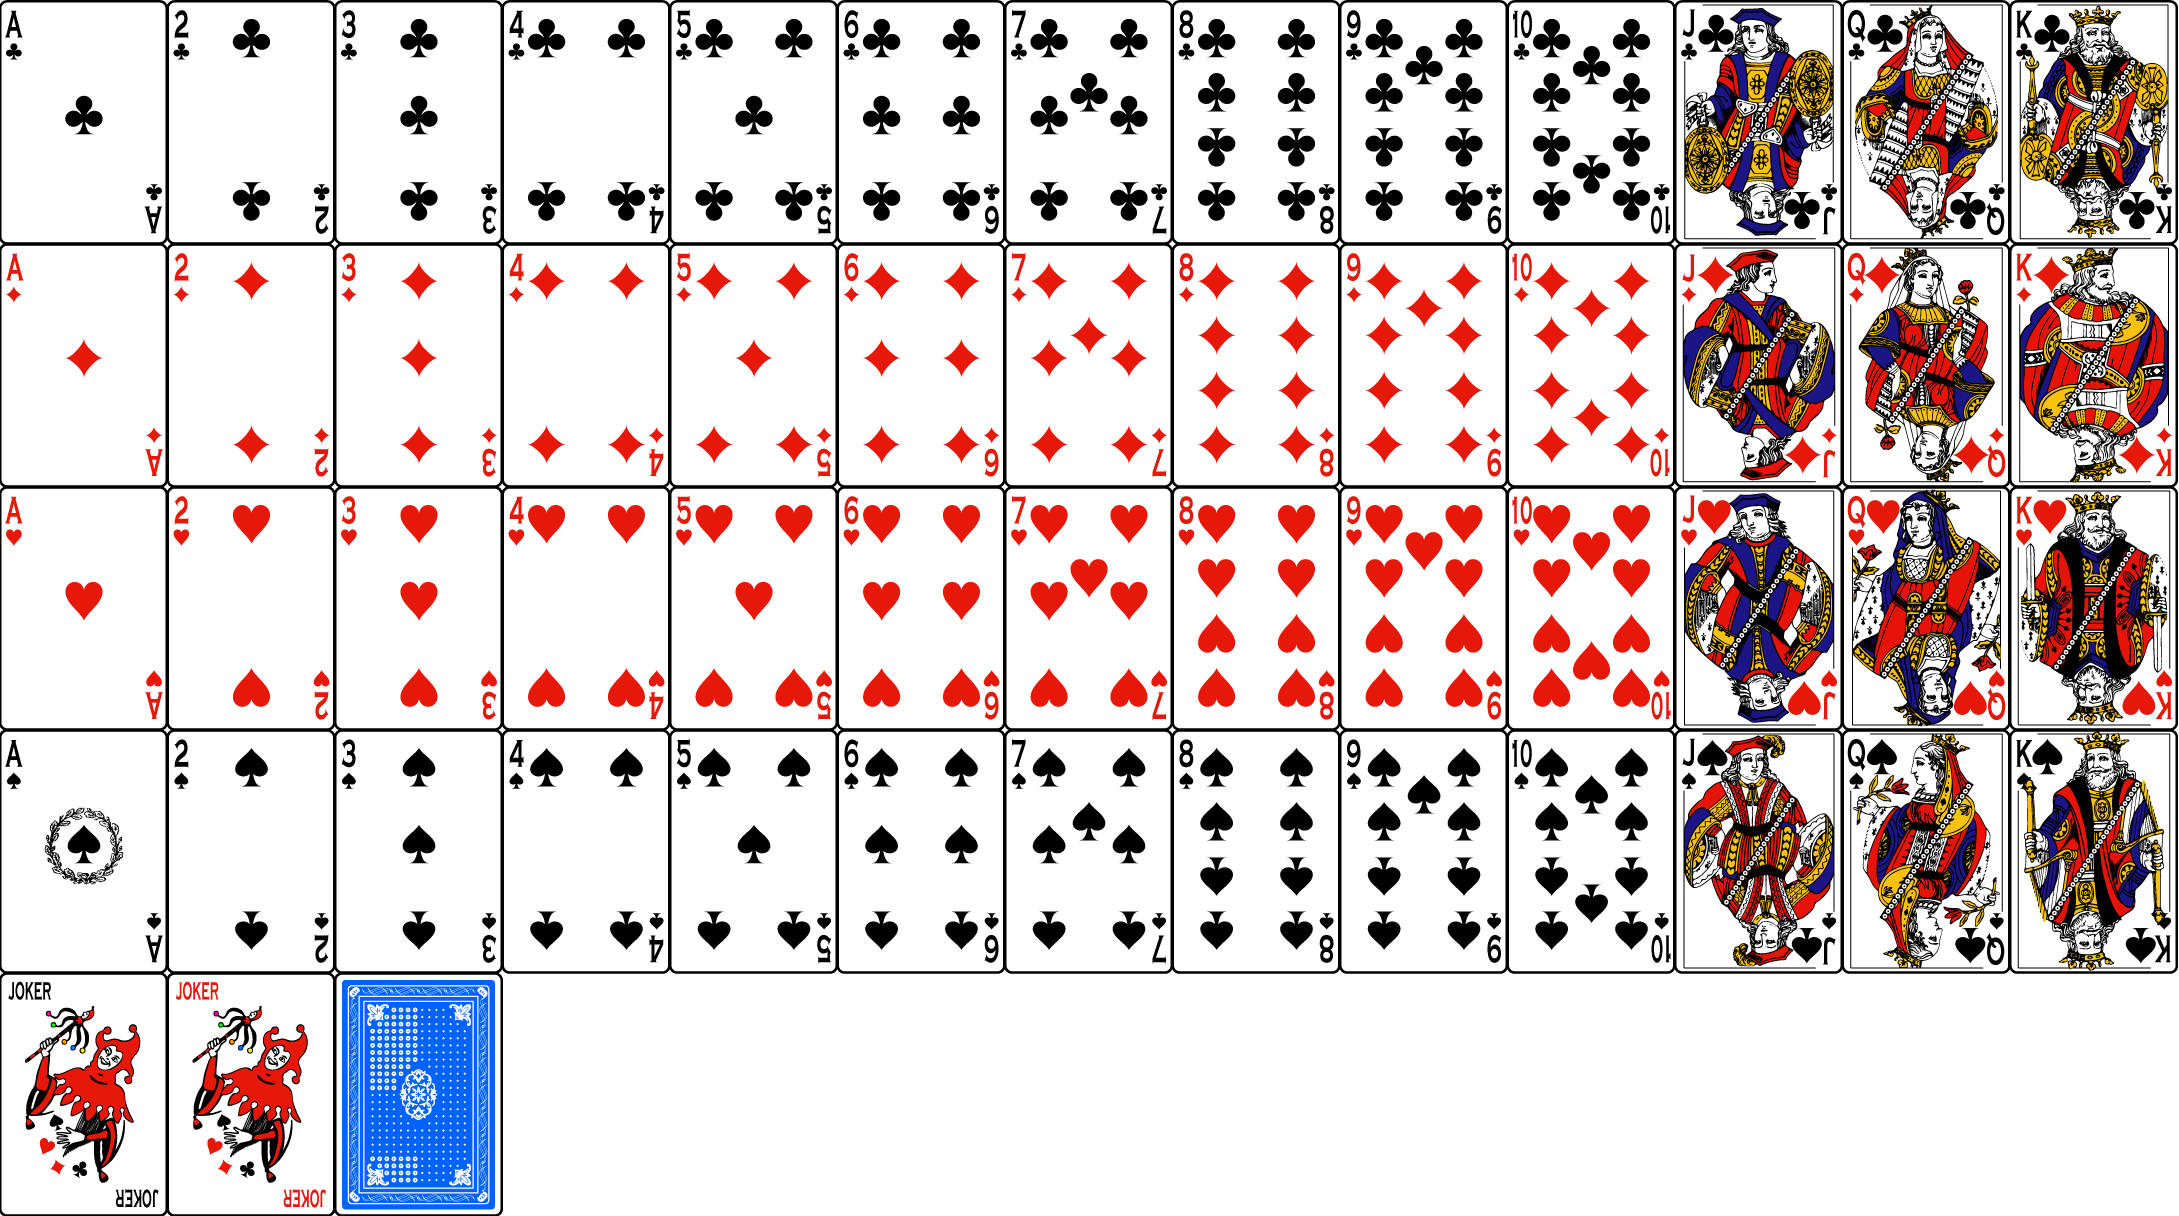
\includegraphics[scale=.34]{cards}
\begin{itemize}
\item Suits: $\clubsuit,\spadesuit,\alert{\vardiamond},\alert{\varheart}$
(club, spade, diamond, heart)
\item Colors: \alert{red}, black
\item Values: $\text{Ace},2,3,4,5,6,7,8,9,10,\text{Jack},\text{Queen},\text{King}$
\end{itemize}
\end{frame}

\begin{frame}{Card Examples}
\begin{itemize}
\item If randomly selected card chosen, calculate\dots
\item $P\left\{\text{Ace}\right\}\only<+->{=\frac{4}{52}}
\only<+->{=\frac{1}{13}}
\only<+->{=P\left\{2\right\}=P\left\{3\right\}
=\cdots=P\left\{\text{King}\right\}}$
\item Could also argue that there are $13$ values, each equally likely
\item $P\left\{\text{not $4$}\right\}\only<+->{=\frac{48}{52}
\only<+->{=\frac{12}{13}}}$
\item $P\left\{\alert{\varheart}\right\}
\only<+->{=\frac{13}{52}}\only<+->{=\frac{1}{4}}
\only<+->{=P\left\{\spadesuit\right\}
=P\left\{\alert{\vardiamond}\right\}
=P\left\{\clubsuit\right\}}$
\item Could also argue that there are four suits, each equally likely
\item A \alert{picture card} a Jack, Queen, or King
\item $P\left(\text{picture card}\right)
\only<+->{=\frac{12}{52}}
\only<+->{=\frac{3}{13}}$
\end{itemize}
\end{frame}

\begin{frame}{Cystic Fibrosis (Exercise 77)}
\begin{itemize}
\item Cystic Fibrosis inherited by $1/2500$ Caucasian
and $1/250000$ non-Caucasian births in North America
\item Everyone has \alert{genotype}
with regard to Cystic Fibrosis gene
\item \alert{Genotype} a sequence of two elements of
$\left\{c,C\right\}$, possibly the same
\item So four possible genotypes $cc,cC,Cc,CC$
\item Individuals with genotype $cc$ \alert{have} Cystic Fibrosis,
\item Individuals with $cC,Cc,CC$ do \alert{not}
\item In other words, anyone with $C$ in either position
does \alert{not} have Cystic Fibrosis
\item $C$ called \alert{dominant} and $c$ called \alert{recessive}
\end{itemize}
\end{frame}

\begin{frame}
\begin{itemize}
\item First letter listed in genotype
inherited from father, second from mother
\begin{example}
An inividual with genotype $cC$ inherited
$c$ from father and $C$ from mother
\end{example}
\item Child receives one gene of Father's genotype,
each with probability $\frac{1}{2}$, similarly for Mother's
\end{itemize}
\end{frame}

\begin{frame}{Example}
\begin{itemize}
\item Suppose Father has genotype~$cC$ and mother has~$CC$
\item Note that neither has Cystic Fibrosis
\item Calculate probability that child will have Cystic Fibrosis
\item Organize information in \alert{Punnett square}:
\[\begin{array}{c|cc}
&c&C\\\hline
C&cC&CC\\
C&cC&CC
\end{array}\]
\item Columns correspond with Father's genes, rows with Mother's
\item Note that \alert{none} of possible child genotypes is $cc$
\item So $0$ the probability that child has Cystic Fibrosis
\end{itemize}
\end{frame}

\begin{frame}{Example}
\begin{itemize}
\item Suppose Father and Mother both have genotype~$cC$
\item Note that neither has Cystic Fibrosis
\item Calculate probability that child will have Cystic Fibrosis
\item Organize information in \alert{Punnett square}:
\[\begin{array}{c|cc}
&c&C\\\hline
C&cC&CC\\
C&cC&CC
\end{array}\]
\item Columns correspond with Father's genes, rows with Mother's
\item Note that \alert{none} of possible child genotypes is $cc$
\item So $0$ the probability that child has Cystic Fibrosis
\end{itemize}
\end{frame}



\end{document}
